% \chapter{Fatigue and Fracture of Steel Structures}
\chapter{钢结构的疲劳与开裂}\label{chp:fatigue-fracture-steel-structures}
% \section{Introduction}
\section{简介}
% This chapter introduces basic principles related to fatigue and fracture in steel bridges, and discusses factors that cause fatigue and fracture. Various available options for repairing observed cracking in steel bridges are also presented. These options are adapted from the Manual for Repair and Retrofit of Fatigue Cracks in Steel Bridges (Dexter and Ocel 2006), and are proposed as a guide for the detailing of repairs and retrofits for fatigue cracks. This chapter only contains summarized information from this manual and thus should not be the only means used to develop specifications needed for the repair and retrofit of fatigue damaged details. Refer to the referenced manual for additional detailed descriptions of the topics, procedures, and examples presented in this chapter. Further, this chapter should be used in combination with other existing codes, specifications, and engineering judgment.
本章介绍了钢桥疲劳断裂的基本原理,讨论了疲劳断裂的产生因素。还介绍了修复钢桥中观察到的裂缝的各种可用选项。这些选项改编自 \bkn*{Manual for Repair and Retrofit of Fatigue Cracks in Steel Bridges} \cite{dexter2008m},建议作为疲劳裂纹修复和改造细节的指南。本章仅包含本手册中的摘要信息,因此不应作为制定疲劳损坏细节维修和改造所需规范的唯一方法。有关本章中介绍的主题、过程和示例的其他详细说明,请参阅参考手册。此外,本章应与其他现有规范和工程判断结合使用。

% \section{Background}
\section{背景}
% Cracks found in steel elements of bridges can usually be attributed to fatigue. Fatigue in metals is described as the process by which cracks initiate and grow under repeated loads. These fatigue cracks can lead to failure if the remaining uncracked section can no longer carry the loads experienced by the structure. In the case of bridge structures, fatigue failure usually occurs as a result of the crack growth that initiates from existing discontinuities. In fatigue, these existing discontinuities are treated as existing cracks. All fabricated steel elements contain discontinuities and most contain high stress concentrations at weld toes. The stress levels causing the failure due to fatigue are usually considerably lower than those that can cause failure under static loading conditions. Fatigue cracks usually form under large amounts of load cycles and worsen with higher stress ranges \cite{fisher1998f}.
桥梁钢构件中发现的裂纹通常可归因于疲劳。金属的疲劳被描述为裂纹在重复载荷下产生和扩展的过程。如果剩余的未开裂部分不能再承受结构所承受的荷载,这些疲劳裂纹会导致结构失效。在桥梁结构的情况下,疲劳失效通常是由于现有的不连续性引发的裂纹扩展而发生的。 在疲劳中,这些现有的不连续性被视为现有的裂纹。 所有制造的钢\gls*{element}都包含不连续性,并且大多数在焊趾处存在高应力集中。由于疲劳而导致失效的应力水平通常远低于在静态负载条件下可能导致失效的应力水平。 疲劳裂纹通常在大量的荷载循环下形成,并随着应力幅的提高而恶化 \cite{fisher1998f}。

% Cracks and discontinuities are expected in steel structures and do not necessarily mean that the member will fail as long as the proper precautions are taken. Most modern structures are redundant and allow for the excess stresses in the cracked members to be redistributed, thus keeping the fatigue crack from propagating any further without intervention. However, it is important to assess tension elements that contain cracks to determine the potential for fracture. Bridges that do not possess redundancy for the stresses to be redistributed, face failure of the entire structure if one of the members were to fail; these members are known as fracture critical members. These structures call for more careful attention, as a fatigue crack can be detrimental to the life of the bridge \cite{fisher1998f}.
裂纹和不连续性在钢结构中是预料之中的,但并不一定意味着采取适当的预防措施,该构件还会失效。大多数现代结构都有一定的冗余度,允许重新分配开裂构件中的过大应力,从而防止疲劳裂纹在没有干预的情况下进一步传播。但是,重要的是评估带裂纹的受拉\gls*{element}以确定断裂的可能性。如果桥梁中的一个构件发生故障,那些不具备冗余度可以重新分配应力的桥梁将面临整个结构的破坏;这些构件被称为断裂临界构件。这些结构需要更加小心,因为疲劳裂纹可能会影响桥梁的\gls*{servicelife} \cite{fisher1998f}。

% Fatigue failure often occurs very suddenly, with little warning; however, the process begins at the onset of the structure’s usage, implying that fatigue is progressive. Another important aspect of fatigue is that it is a local phenomenon, occurring in areas of high stresses and strains due to load transfer, abrupt changes in geometry, residual stresses, and material imperfections. The damage caused by fatigue is permanent and is not reversible. Fatigue cracks exist in many structures, but not all of them are critical; certain criteria must be met before the cracks are detrimental to the structural element. Fracture, separation of a component into two or more parts, occurs once the remaining uncracked portion of the member can no longer handle the stresses and strains \cite{stephens2000m}.
疲劳失效往往发生得非常突然,几乎没有任何征兆;然而,这个过程是从结构开始使用开始的,这意味着疲劳是渐进的。关于疲劳的另一个重要方面是它是一种局部现象,发生在由于荷载转移、几何形状突化、残余应力和材料缺陷导致的高应力应变区域。疲劳造成的损害是永久性的,不可逆。疲劳裂纹存在于许多结构中,但并非所有都是关键的;在裂缝能对结构\gls*{element}造成危害之前必须符合某些条件。 一旦构件剩余的未开裂部分不再能承受应力和应变,就会发生断裂,即一个\gls*{component}分离成两个或多个部分 \cite{stephens2000m}。

% The entire fatigue process includes the nucleation (formation) of a fatigue crack, crack propagation (growth), and final fracture (failure). The nucleation of a fatigue crack takes place at the microscopic level, dealing primarily with the microstructure of the material. Discontinuities are common sites of crack nucleation and include persistent slip bands, inclusions, pores, second-phase particles, corrosion pits, voids, and twin and grain boundaries. However, cracks primarily tend to nucleate along slip lines in the direction of planes of maximum shear \cite{stephens2000m}.
整个疲劳过程包括疲劳裂纹形成、裂纹扩展和最终断裂(失效)。 疲劳裂纹的形成发生在微观层面,主要涉及材料的微观结构。 不连续性是裂纹形成的常见部位,包括持久性滑移带、夹杂物、孔隙、第二相颗粒、腐蚀坑、空隙以及孪晶和晶界。 然而,裂纹主要倾向于沿着最大剪切平面方向的滑移线形成 \cite{stephens2000m}。

% Once a fatigue crack forms and continues to undergo repeated loading, it tends to coalesce and grow along the plane of maximum tensile stress range. The crack will grow with each load cycle, even if only by a small amount. As the cracked member is loaded, the crack will open causing an increase in stress at the crack tip; this consequently drives the crack to grow even larger. Fatigue crack growth is broken up into two stages; Stage 1 and Stage 2, as seen in the \cref{fig:crack-growth}. Stage 1 refers to the growth in the direction of the principal shear plane, whereas Stage 2 refers to the growth along the plane of maximum principal tensile stress. Fatigue cracks tend to grow transcrystalline (through grains), but some fatigue cracks can grow intercrystalline (along grain boundaries). Crack growth mechanisms include striation formation, microvoid coalescence (MVC), and microcleavage. Striations are microscopic “ripples” that are representative of the fatigue cycles experienced by the element. Striation can be used to investigate the rate of crack growth and are very useful in forensic studies. MVC involves the formation, growth, and joining of microvoids during plastic deformation. Microcleavage is a fracture along specific crystallographic planes and tends to be a brittle fatigue mode \cite{stephens2000m}.
一旦疲劳裂纹形成并继续承受往复荷载,它就会沿着最大拉应力范围的平面合并和扩展。 裂纹会随着每个荷载循环而增长,即使只是少量增长。当有裂纹的构件被加载时,裂纹会张开,导致裂纹尖端的应力增加,因此,这会促使裂缝变得更大。疲劳裂纹扩展分为两个阶段:阶段 1 和阶段 2,如\cref{fig:crack-growth} 所示。 阶段 1 是指在主剪切面方向上的增长,而阶段 2 是指沿最大主拉应力平面的增长。 疲劳裂纹倾向于跨晶(穿过晶粒)生长,但一些疲劳裂纹可以在晶间(沿晶界)生长。 裂纹增长机制包括条纹形成、微孔聚结 (MVC) 和微裂解。 条纹是微观“波纹”,代表元件所经历的疲劳循环。 条纹可用于研究裂纹的增长速度,在法医研究中非常有用。 MVC 涉及塑性变形过程中微孔的形成、生长和连接。 微裂纹是沿着特定晶面的断裂,往往是一种脆性疲劳模式 \cite{stephens2000m}。

\begin{figure}
  % \includegraphics[width=\linewidth]{graphic-file}
  % \caption{Schematic of Stages 1 and 2 of fatigue crack growth. \cite{stephens2000m}}
  \caption{疲劳裂纹扩展阶段 1 和 2 的示意图\cite{stephens2000m}}
  \label{fig:crack-growth}
\end{figure}

This section presents only a brief and very general summary of the fatigue process, but it is important for the practicing engineer to understand the principles of the fatigue damage process in order to be proficient in fatigue design.

Minimizing fatigue cracks can be achieved by first avoiding the use of known details that have proven to have low resistance to fatigue. Fatigue cracks can also be reduced by the use of better fabrication and welding processes that lower inherent defects and also allocate for the detection and repair of such cracks before the bridge is opened to the public. In-service inspection is necessary to discover new fatigue cracks and monitor existing ones. Once cracks are located through the inspection process, it is necessary to perform an assessment to determine the risk of fracture. Furthermore, for the proper repair methods to be implemented, the cause and type of crack need to be determined \cite{fisher1998f}.

% Several methods exist for determining the fatigue resistance of a detail; these include: nominal stress approach, hot-spot stress approach, and fracture mechanics.
有几种方法可用于确定细节的抗疲劳性; 其中包括:标称应力法、热点应力法和断裂力学。

\subsection{Nominal Stress Approach}
This design approach is a simple way to determine the fatigue resistance of a detail using equations for bending
and axial loads to compute the nominal stress near a weld toe. Test data from full-scale fatigue tests are needed in
order to utilize this design method. Stress ranges (S) versus the number of cycles to failure (N) curves are developed from the test data. The curves are also grouped into categories to aid in organizing the details according to their
fatigue resistance. \cref{fig:s-n-curve} shows the S-N curves as used in AASHTO specifications. The detail categories reflect
and account for the variations in the combined geometric and local notch stress concentrations. Each category has a
constant-amplitude fatigue limit (CAFL), also referred to as threshold (CAFT). Stress ranges that fall below the
CAFL are not expected to exhibit any fatigue failures during constant-amplitude test.

Most bridges with a service life of 75 years are designed as having an infinite-life, no occurrence of fatigue
cracking. In the AASHTO LRFD Bridge Design Specifications (LRFD Specifications), the fatigue design live load is
taken as 0.75 times the HS20 for finite load-induced fatigue life and 1.5 times the HS20 for infinite load-induced
fatigue life. This fatigue load is used to calculate the nominal stress ranges to be used with the S-N curves. If the
resulting nominal stress range is less than half of the CAFL, it is assumed the bridge is designed for infinite life. This
ensures that the fatigue limit-state stress range is below the CAFL. The fatigue limit-state is the stress range in which
0.01 percent of the test data exceeds the CAFL. (AASHTO 2012)

\begin{figure}
  % \includegraphics[width=\linewidth]{s-n-curve}
  % \caption{S-N curves used in AASHTO, AISC, AWS, and AREMA specifications. (AASHTO 2012)}
  \caption{AASHTO、AISC、AWS 和 AREMA 规范中使用的 $S$-$N$ 曲线 \cite{aashto2012l}}
  \label{fig:s-n-curve}
\end{figure}


\subsection{Hot-Spot Stress Approach}
This approach is similar to the nominal stress approach, however the S-N curves are based on the geometric
stress ranges, also known as hot-spot stresses. This process is beneficial in instances where the nominal stress
approach breaks down, such as offshore tubular structures where the fatigue resistance is heavily dependent on the
geometry of the tubes. Using this design process involves determining the stress concentration factor using
parametric equations or finite element analysis. Disadvantages arise with the variability of different hot-spot
definitions, varying baseline S-N curves, and difficulties with the CAFL.

\subsection{Fracture Mechanics Approach}
In the case of bridge structures, this is the most complex approach and tends to be difficult to implement during
the bridge design process. The fracture mechanics approach is divided into two main categories: Linear Elastic
Fracture Mechanics (LEFM) and Plastic Fracture Mechanics (PFM). LEFM is used when remotely applied stresses
are in elastic ranges. It should be noted that at the crack tip, a stress singularity is always present and stresses tend to
approach infinity. In the case of LEFM, the rate of crack growth is related to stress ranges, while in the case of PFM,
rate of crack growth needs to be related to a parameter related to energy dissipation or plastic strain (Azizinamini and
Radziminski 1989).

For the case of LEFM, the Paris Law, shown in Equation 7.1, can be useful in determining the crack growth rate
for many engineering applications.

\section{Crack Detection Techniques}
Cracks are not always obvious to the human eye and can be difficult to locate at times. There are several
methods in practice to aid in the detection of cracks, two of which are dye penetrant and magnetic particle inspection.

Dye penetrant consists of three parts; cleaning the area of a suspected crack, application of a liquid dye, and
finally the application of a white developer. Figure 7.3 shows a crack exposed using a red dye penetrant.

\begin{figure}
  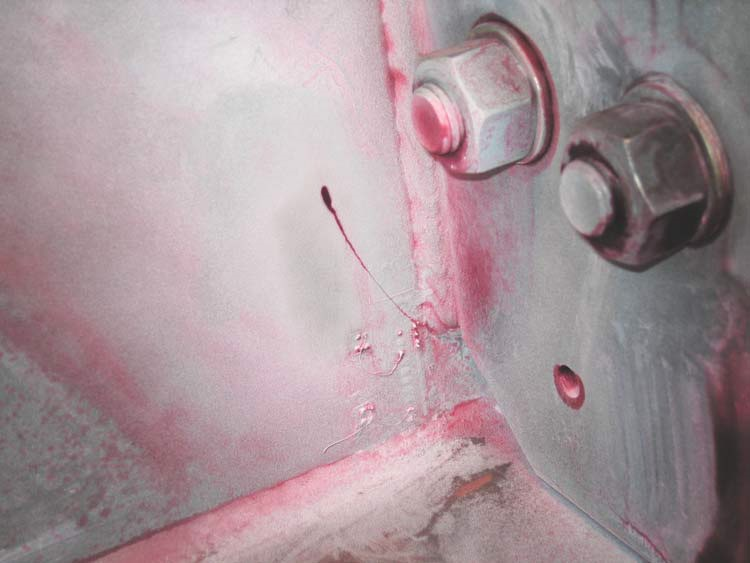
\includegraphics[width=0.5\linewidth]{crack-exposed.jpg}
  \caption{Crack exposed using a red dye penetrant}
  \label{fig:crack-exposed}
\end{figure}

Magnetic particle inspection works by inducing a magnetic field using a handheld device around a crack. The
magnetic field is disrupted at the crack and a concentration of a magnetic field results. A fine iron powder is
sprinkled over the area of interest and is attracted to the magnetic field, exposing the crack.

\section{Repair and Retrofit Methods}
This section presents several methods for the repair and retrofit of fatigue critical details. Such techniques can be
categorized as surface treatments, repair of through-thickness cracks, and connection or global structure modification
to reduce the causes of cracking.

\subsection{Surface Treatments}
Surface treatments are usually performed on weld toes to increase the fatigue strength of uncracked welds. Such
treatments, including grinding, gas tungsten arc (GTA), and impact treatments, aim to improve the weld geometry in
order to reduce stress concentrations, remove discontinuities, and/or reduce residual tensile stresses.

\subsection{Reshape by grinding}
Grinding can be used as an effective measure for increasing the fatigue life of the weld toe by removing portions
of the weld that contain small cracks. Grinding has proven more effective on larger welds in structures such as
offshore structures with large tubular joints. It should be noted that grinding is ineffective against microcracks
because the process tends to create new microcracks as it removes the existing ones. Two types of grinding methods
are commonly used; disc grinding (\cref{fig:disc-grinding}) and burr grinding (\cref{fig:burr-grinding}), and both have advantages and
disadvantages. Disc grinding can be more effective at removing the weld material with faster speeds; however, the
operator needs to use caution to avoid gouging the metal or removing too much of the weld material. Burr grinding is
typically easier to operate and works in more confined spaces than disc grinding. (Gregory et al. 1989)

\begin{figure}
  % \includegraphics[width=\linewidth]{graphic-file}
  \caption{Disc grinding}
  \label{fig:disc-grinding}
\end{figure}

\begin{figure}
  % \includegraphics[width=\linewidth]{graphic-file}
  \caption{Burr grinding}
  \label{fig:burr-grinding}
\end{figure}

\subsection{Gas Tungsten Arc (GTA) or Plasma Remelting}

GTA aims to reduce the stress concentrations at the weld toe and also remove slag intrusions. This process
involves melting a small volume of the weld toe and base material using tungsten electrodes. In order for this
process to effectively increase the weld’s fatigue life, the operator needs great skill, which consequently increases the
cost of this process.


\subsection{Impact treatments}

Compressive residual stresses can be induced around the weld toe using impact treatments. These compressive
stresses reduce the effective tensile stress range, extending the fatigue life of welds. Since impact treatments enhance
the weld profile and residual stresses, the process can only effect stresses transverse to the impacted weld. Thus,
impact treatments are most effective on transversely-loaded welds and have no effect on longitudinally-loaded welds.
The most common types of impact treatments include air hammer peening and ultrasonic impact treatment.

Air hammer peening utilizes an air-powered hammer with a blunt tip that plastically deforms the weld toe. This
is simple method that can increase the fatigue resistance by at least one detail category. For instance a category C detail could be improved to category B detail. Air hammer peening reduces the number of slag intrusions but at the
same time creates lap-type defects. These lap-type defects can be reduced by light grinding following the peening.
(Hausammann et al. 1983)

Ultrasonic impact treatment (UIT) has proven to be more effective than hammer peening by using low-amplitude
and high frequency displacements. However, UIT can be more costly as it is still a proprietary method. (Tryfyakov
et al. 1993; Roy et al. 2003)

\subsection{Hole Drilling}

Hole drilling is the most widely used method for the repair of fatigue cracks. The process involves drilling a hole
at the tip of the crack (propagating end). The larger the hole, the more effective it is at arresting the fatigue crack
from propagating, as long as the hole is not detrimental to the stiffness of the member. Holes should not be made
smaller than 1 in. in diameter as holes smaller than this tend to be ineffective. Holes should be sealed against
corrosion and plugged to hide the hole from the public. Equations have been developed in order to simplify the
process of hole size selection for in-plane fatigue as seen below. (Fisher et al. 1980)
\begin{align}
  \frac{\Delta K}{\sqrt{\rho}} & \leqslant 10.5\sqrt{\sigma_\text{y}}\\
  \Delta K& = S_\text{r}\sqrt{\uppi a} 
\end{align}
\begin{EqDesc}{\Delta K}
  \item[\Delta K] stress intensity factor
  \item[\rho]radius of the hole
  \item[\sigma_\text{y}]yield stress of material
  \item[S_\text{r}]nominal stress range at crack tip
\end{EqDesc}

At the tip of cracks , dingularity exist and stresses approach infinity. Drilling eliminates the high stress concenteration and prevents the further crack growths.

\subsection{Vee-and-Weld}
This method is best for long, through-thickness cracks. The process includes removing the material along the
crack in the shape of a V, and then filling the grove with weld material. The groove can be made using several
methods, the preferred being air arc gouging. Grinding can also be done, but it tends to smear the crack path making it harder to detect the crack and follow its path. Other methods need to be used in addition to vee-and-weld repairs in
order to reduce the stress ranges at the location of the repair. This is necessary because the vee-and-weld repairs only
have a fatigue life that is equal to that of the original uncracked weld. (Dexter et al. 2003)

\subsection{Adding Doubler/Splice Plates}

Doubler plates can be added at crack locations to increase the cross-sectional area and therefore reduce the stress
ranges experienced by that section. (See Figure 7.6.) Doubler plates are designed to restore the section properties of
the cracked section to the uncracked state using design processes identical to those of field splice connections.

\begin{figure}
  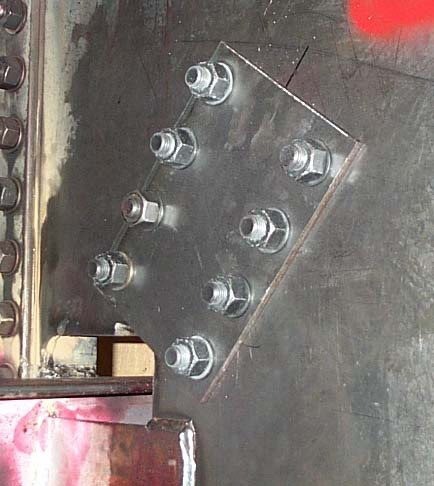
\includegraphics[width=0.5\linewidth]{bolted-double-plate-repair.jpg}
  \caption{Photo of bolted doubler plate repair}
  \label{fig:bolted-double-plate-repair}
\end{figure}

\subsection{Posttensioning}
Posttensioning methods that are applied to cracked sections can prolong the fatigue life of the structure. Post-
tensioning induces forces on the cracked section that put the effective stress ranges into compression, keeping the
crack closed and unable to propagate. It is recommended to drill a hole at the crack tip in addition to one of the
various types of posttensioning that is to be used.


\subsection{Detail Modification}
Detail modification is used when it is necessary to lower the effective stress range in order to repair the cracked
section. This can be achieved in a number of ways, among them increasing the cross-sectional area, changing
connection geometry, or eliminating sharp corners from details.

\section{Fatigue Due to Secondary Stresses}

Secondary stresses can arise when a structure is designed as a series of individual components and the designer
does not account for the global system behavior. These stresses can cause unexpected fatigue cracking. This section
discusses these stresses and the methods used to repair the fatigue cracks that form under secondary stresses.



\subsection{Out-of-Plane Distortion}
Differential displacements between girders and lateral bracing elements introduce fatigue to the web-gap regions
of the girders. This phenomenon causes highly localized bending of the web-gap, as shown in Figure 7.7, causing
fatigue cracks. In order to properly repair the fatigue cracks the out-of-plane bending needs to be reduced or
eliminated. It is important to note that web-gap fatigue retrofits need to maintain symmetry.

\begin{figure}
  % \includegraphics[width=\linewidth]{graphic-file}
  \caption{Web-gap fatigue mechanism from displacement continuity. Top: Differential girder displacements cause a force couple to develop within the diaphragm. Bottom: Zoomed view of web-gap deformation girder displacement.}
  \label{fig:web-gap-fatigue}
\end{figure}

\subsubsection{Repair Methods Specific to Out-of-Plane Distortion}
\paragraph{Hole Drilling}
This method can be effective at reducing the crack growth but not eliminating the cause of the fatigue. See the
above section on hole drilling for additional details; however, note that the hole sizing equations were developed for
in-plane fatigue and may not have the same effect on out-of-plane distortion induced fatigue.
\paragraph{Diaphragm or Crossframe Removal}
Diaphragms and crossframes transfer the secondary forces between girders when differential displacement of the
girders occurs. Removing these members eliminates the causes of the fatigue-induced cracks in the web-gaps.
However, several issues of concern have arisen from the removal of such bridge elements. It has been shown that the
removal of the lateral bracing elements can be detrimental to the structure when not properly removed. In negative
moment regions, the lateral bracing keeps the compression flange from buckling. Also, if the diaphragms and
crossframes were removed, as the bridge deck needs to be replaced, no lateral bracing would exist to keep the girders
stable when the deck is removed. Some studies show that crossframes are effective to some extent in distributing the applied traffic loads (Brakke 2001; Flemming 2001). However, extensive investigation of crossframes indicated that
it is the stiffness of the deck that is mainly responsible for distribution of truck loads between girders, and that
crossframes are not contributing to load distribution. (Azizinamini et al. 1995a; Azizinamini et al. 1995b)
\paragraph{Diaphragm Repositioning}
It has been shown that lowering diaphragms closer to the bottom flange of the girders (in negative moment
regions) and reducing the number of connecting bolts can reduce the effective stress range. This was seen in a case
study of I-35W Bridge over the Mississippi River in Minneapolis, Minnesota. (Bergson 1998) See Figure 7.8.

\begin{figure}
  % \includegraphics[width=\linewidth]{graphic-file}
  \caption{Schematic of diaphragm repositioning retrofit specified on Minnesota Bridge.}
  \label{fig:diaphragm-reposition-retrofit}
\end{figure}

\paragraph{Bolt Loosening}
Loosening the connection bolts can reduce the effect of the out-of-plane displacements. The holes are specified
to be larger than the size of the bolts, and this extra space negates the effects of small differential displacements.
However, the effectiveness of loosening the bolts is limited to the extra space provided by the oversized holes and
whether or not the holes are in bearing due to misaligned connection plates. Additional measures are needed to
ensure that the loosened nut does not fall off of the bolt due to vibrations of the structure. (Wipf et al. 1998)

\paragraph{Web-Gap Stiffening}
Permanently attaching the connection plate to the girder flange can reduce or eliminate the effects of out-of-plane
displacements. Several types of methods exist for the attachment of the connection plate to the girder flange: all
welded, all bolted, welded and bolted, adhesives, and nails.

\paragraph{Welded Attachment}
The all-welded retrofit for connection plates can be difficult to implement. For instance, the welded connection
itself can cause fatigue cracks. (Keating et al. 1996) In addition, it can be very difficult to properly weld high
strength steels as well as flanges that are embedded in concrete. Although AASHTO now requires transverse welds
or bolted connections on both the girder flanges for the positive attachment of the connection plate, the all-welded
attachment retrofit has rarely been specified for reasons previously mentioned. (AASHTO 2012) Figure 7.9 shows a
fillet welded connection plate to girder detail.

\begin{figure}
  % \includegraphics[width=\linewidth]{graphic-file}
  \caption{Connection plate-to-girder fillet weld detailing. (Keating 2001)}
  \label{fig:plate-to-girder-fillet-weld}
\end{figure}

\paragraph{Bolted Connections}
The connection plate can be bolted to the girder flange using angles or sections. It is important to properly size
the angles and tee sections and number the amount of bolts needed in order to provide for the proper stiffness of the
section. Bolted tee sections are preferred over double angles because they provide greater stiffness. (Fisher et al.
1990) See Figure 7.10.

\begin{figure}
  % \includegraphics[width=\linewidth]{graphic-file}
  \caption{Schematic of concrete deck haunch removal to allow for bolt installation. (Keating 2001)}
  \label{fig:concrete-dec-haunch-removeal}
\end{figure}

\paragraph{Hybrid Connections}
These types of connections utilize both welded and bolted connections and may be more beneficial in areas with certain clearance issues
\subparagraph{Adhesives}
Adhesives become attractive when short-term positive attachments are needed. They can be less expensive than
the bolted or welded options because they do not require the removal of any concrete. (Hu 2005) See \cref{{fig:stiffening-retrofit}}.

\begin{figure}
  % \includegraphics[width=\linewidth]{graphic-file}
  \caption{Work plan for stiffening retrofit of web-gaps with adhesives. (Hu 2005)}
  \label{fig:stiffening-retrofit}
\end{figure}

\subparagraph{Nails}
Powder-actuated fasteners are the newest and perhaps the best alternative for stiffening web-gaps. These
fasteners are made of high strength materials and are propelled into the girder flanges using explosive discharges.
Concern has been raised on the possible fatigue issues of these powder-actuated nails, but research has shown that the
fasteners perform adequately with little detriment to the members. Due to dimensional issues, nails are only used for
the flange connection while bolts are used for attachments to the connection plate as shown in \cref{{fig:web-gap-retrofit-nails}}. When
determining the number of nails to use, it is imperative that the manufacturer’s recommended nail shear resistance be
used. (Niessner and Seeger 1999)

\begin{figure}
  % \includegraphics[width=\linewidth]{graphic-file}
  \caption{Work plan for web-gap retrofit using nails.}
  \label{fig:web-gap-retrofit-nails}
\end{figure}

\paragraph{Web-Gap Softening}
Web-gap softening entails the removal of portions of material to make the web-gap more flexible. See \cref{fig:web-gap-softening}.

\begin{figure}
  % \includegraphics[width=\linewidth]{graphic-file}
  \caption{ Work plan for web-gap softening used on Poplar Street Bridges in East St. (Koob et al. 1998)}
  \label{fig:web-gap-softening}
\end{figure}

A portion of the connection plate can be removed in order to increase the size of the web-gap and therefore
reduce the stresses due to out-of-plane distortion. After flame cutting the connection plate it is important to grind the
portion of the web smooth and flush where the connection plate was previously attached.

A simpler and faster approach to softening the web-gap would be drilling large holes in the web of the girder
close to the web-gap. See Figure 7.14. This process is much like the smaller hole retrofits discussed earlier; however,
the larger diameter holes are able to capture several cracks as opposed to the “Swiss cheese” method of numerous
smaller holes.

\begin{figure}
  % \includegraphics[width=\linewidth]{graphic-file}
  \caption{Schematic of typical large diameter hole retrofit. (Koob and McGormely 1998)}
  \label{fig:large-diameter-hole-retrofit}
\end{figure}

\subsection{Tie Girder/Floor Beam Connection}
Tied arch bridges exhibit a specific type of web-gap fatigue in the connections between the floor beams and the
tie girders. This fatigue arises from the displacement incompatibility between the floor beams that are composite
with the bridge deck and the non-composite tie girder. The mode of deformation is illustrated in \cref{fig:girder-floor-beam-cracking}.
Several retrofits have been implemented in the field and subsequently studied. These studies are presented in the
report from which this section has been adapted. (Dexter and Ocel 2008)

\begin{figure}
  % \includegraphics[width=\linewidth]{graphic-file}
  \caption{Schematic of tie girder to floor beam cracking driving force}
  \label{fig:girder-floor-beam-cracking}
\end{figure}

\subsection{Cantilever Bracket Cracking}
Floor beam cantilevered brackets are used on bridges with large deck overhangs and can be susceptible to
secondary stress fatigue. Several retrofit options exist for reducing the displacement incompatibility of the girder and
floor beams. These retrofits deal mainly with the modification of the tie plates that span over the girders. The main
idea is to either remove any positive attachments between the girders and tie plates or add spacer plates to create a
gap between the elements. \cref{fig:two-girder-cantilever-bracket,fig:plate-detail-deformation-mode,fig:retrofit-tie-plate-cracking} show the deformation modes and possible retrofit options.

\begin{figure}
  % \includegraphics[width=\linewidth]{graphic-file}
  \caption{Typical cross-section of a two-girder bridge with cantilever bracket outriggers.}
  \label{fig:two-girder-cantilever-bracket}
\end{figure}

\begin{figure}
  % \includegraphics[width=\linewidth]{graphic-file}
  \caption{Zoomed-in view of tie plate detail (left) and deformation mode that causes cracking (right)}
  \label{fig:plate-detail-deformation-mode}
\end{figure}

\begin{figure}
  % \includegraphics[width=\linewidth]{graphic-file}
  \caption{Retrofit of tie plate cracking through addition of spacer plates.}
  \label{fig:retrofit-tie-plate-cracking}
\end{figure}


\section{Retrofit Validation of Secondary Stress Fatigue}
Due to the unknown nature of retrofitting web-gap fatigue, it is necessary to validate particular retrofits before
retrofitting an entire bridge. The simplest plan to validate a particular retrofit is to first instrument an uncracked
detail, then perform the necessary retrofit and validate whether or not the retrofit adequately lowered the stress ranges
and out-of-plane displacements. Typical instrumentation includes the use of strain gauges and/or displacement
measurement devices.

Strain gauges are very common and effective instruments used to determine the effective stress ranges of bridge elements. Strain gauges can be either spot welded or glued to the element of interest. \cref{fig:recommended-strain-gauge-placement} shows preferable strain gauge layouts for retrofit validation.

\begin{figure}
  % \includegraphics[width=\linewidth]{graphic-file}
  \caption{Recommended strain gauge placement for retrofit validation. Bottom: Strain gauge placement for out-of-plane distortion. Top: Strain gauge placement for floor beam/tie girder connection or beam cope cracking}
  \label{fig:recommended-strain-gauge-placement}
\end{figure}

Measuring the displacements has become the preferable method for validating retrofits because displacement
measurements are quicker and more cost-effective than strain measurements. That displacement gauges are only
usable for stiffening retrofits should be taken into account. Two common types of displacement measuring devices
are linear variable differential transformers (LVDTs) and dial gauges. \cref{fig:web-gap-displacement-instrumentation} shows a schematic for the
placement of the devices to measure the web-gap displacement. It should be noted that maximum distortion-induced
fatigue strains/stresses do not always correlate with the largest values of differential deflection, and an
instrumentation plan based primarily on displacements may not capture the whole picture.

In the final analysis, however, the choice of instrumentation to validate the retrofit type is context sensitive. The
designer must select an instrumentation type that best matches the retrofit type.

\begin{figure}
  % \includegraphics[width=\linewidth]{graphic-file}
  \caption{Recommended web-gap displacement instrumentation.}
  \label{fig:web-gap-displacement-instrumentation}
\end{figure}

\section{Load Controlled Fatigue Crack Repair}

\subsection{Coverplates}
Several methods have been explored in the retrofitting of coverplates including grinding, air hammer peening,
GTA, and bolted splice plates. Grinding has proven ineffective and therefore is not recommended. Bolted splice
plates are an effective option for girders with severed flanges and in instances in which the aforementioned methods
are undesirable. See \cref{fig:detail-splice-plate-retrofit-cracked-coverplate}.

\begin{figure}
  % \includegraphics[width=\linewidth]{graphic-file}
  \caption{Detailing of splice plate retrofit for cracked coverplate details.}
  \label{fig:detail-splice-plate-retrofit-cracked-coverplate}
\end{figure}

\subsection{Eyebars and Hangers}
Eyebars are long slender bars or rods with forged eyes at the ends and are commonly used as tension members in
truss bridges. Hangers are vertically-oriented tension members supporting load. Both eyebars and hangers are often
the sole component supporting the particular tensile load and are therefore usually classified as fracture critical
members and inherent flaws can lead to fatigue cracks.

Assessing the integrity of eyebars, especially in old truss bridges, is very difficult. An example of eyebar with
extensive corrosion is shown in \cref{fig:corrosion-eyebar-connection}.

\begin{figure}
  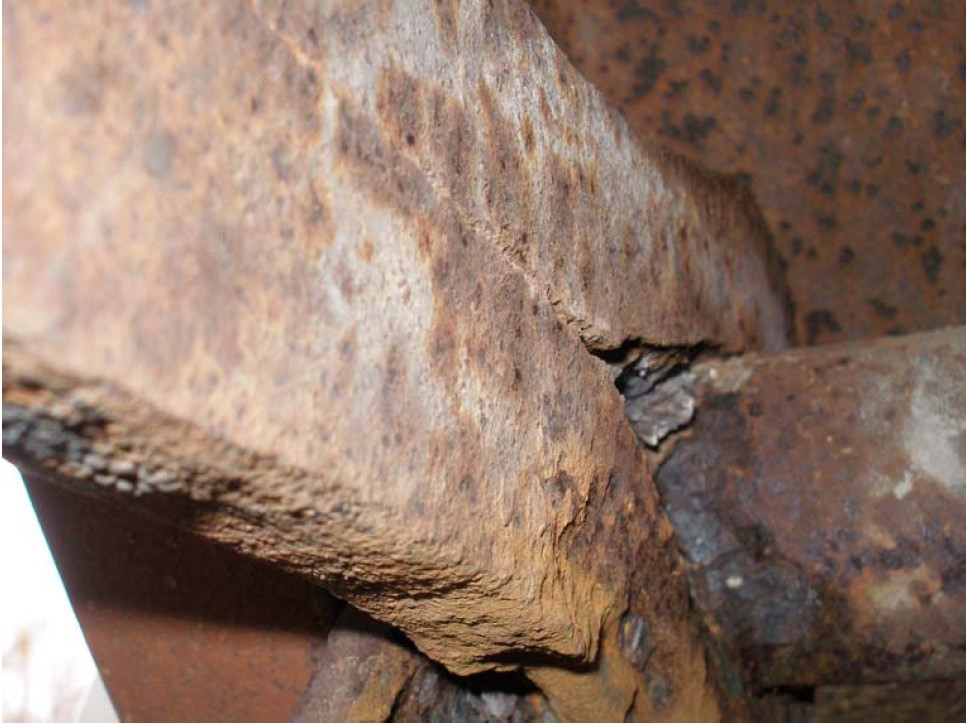
\includegraphics[width=0.5\linewidth]{corrosion-eyebar-connection.jpg}
  % \caption{Corrosion of eyebar connection.}
  \caption{Corrosion of eyebar connection.}
  \label{fig:corrosion-eyebar-connection}
\end{figure}

In the case of truss bridges, it is recommended to add, rather than replace truss members. Removing even single
truss member or connection could easily lead to bridge failure. In retrofitting many existing old truss bridges,
extensive corrosion of eyebars in tension could be addressed by adding additional tension members, while keeping
the existing ones in place. \cref{fig:retrofit-option-eyebar-connection} shows a possible retrofit alternative for eyebars in tension in existing truss
bridges. (Azizinamini 2002)

\begin{figure}
  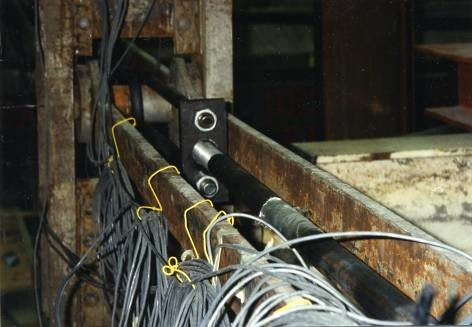
\includegraphics[width=0.5\linewidth]{retrofit-option-eyebar-connection.jpg}
  \caption{Retrofit option for eyebar connection.}
  \label{fig:retrofit-option-eyebar-connection}
\end{figure}

\subsection{Temporary Tack Welds}
Tack welds used to temporarily hold members in place during construction can be sources of concern for fatigue
cracks. Fatigue cracks tend to form at the ends of the tack welds and then propagate into the base metal. The most
susceptible types of tack welds are longitudinal, and those located at the end of tack-welded members. Tack welds
can be removed using grinding methods.


\subsection{Connection Angles}
Connection angles used to connect diaphragms to girder webs are susceptible to fatigue cracking due to
differential girder displacements. See \cref{fig:deformation-mode-coneection-angles}. The thickness of such angles needs to be reduced in order to
reduce the flexural rigidity of the elements and negate the causes of the differential girder displacements. The
following equation helps determine the proper angle thickness to prevent cracking. (Dexter and Fisher 1999)
\begin{equation}
  t\leqslant 12\left(\frac{g^2}{L}\right)
\end{equation}
\begin{EqDesc}{g}
  \item[t] angle thickenss
  \item[g] bolt gauge
  \item[L] distance between girders
\end{EqDesc}

\begin{figure}
  % \includegraphics[width=\linewidth]{graphic-file}
  \caption{Deformation mode of connection angles due to displacement compatibility.}
  \label{fig:deformation-mode-coneection-angles}
\end{figure}

\subsection{Web Gusset Plates}
Another source of fatigue cracks are web gusset plates, which can experience fatigue damage due to weld root
defects and locations of intersecting welds. Intersecting welds can be retrofitted by coring holes at the intersections;
this will not only remove the intersecting welds, but also reduce the web constraint. See \cref{fig:deep-girder-web-gusset,fig:retorfit-detail-gusset-plates}.

Fatigue cracks have also been found to initiate from the ends of the gusset plates and propagate into the girder
webs. This issue can be solved using impact treatments or grinding of the weld termination. See \cref{fig:detailing-crack-site2-retrofit}.

\begin{figure}
  % \includegraphics[width=\linewidth]{graphic-file}
  \caption{Typical cross-section of a deep girder bridge (top) and plan view of the web gusset detail (bottom).}
  \label{fig:deep-girder-web-gusset}
\end{figure}

\begin{figure}
  % \includegraphics[width=\linewidth]{graphic-file}
  \caption{Retrofit detail for gusset plates with intersecting welds. (Crack Site \#1)}
  \label{fig:retorfit-detail-gusset-plates}
\end{figure}

\begin{figure}
  % \includegraphics[width=\linewidth]{graphic-file}
  \caption{Detailing of crack site \#2 retrofit}
  \label{fig:detailing-crack-site2-retrofit}
\end{figure}

\subsection{Longitudinal Stiffeners}
Fatigue cracks can form at the butt welds of longitudinal stiffeners, primarily due to poor workmanship and
inherent defects of the welds. Drilling a large diameter hole into the longitudinal stiffener located next to the girder
has proven to keep the crack from developing into the girder web. See \cref{fig:work-plan-butt-weld-retrofit}.

\begin{figure}
  % \includegraphics[width=\linewidth]{graphic-file}
  \caption{Work plan of longitudinal butt weld retrofit.}
  \label{fig:work-plan-butt-weld-retrofit}
\end{figure}

\subsection{Coped Beam Ends}
Fatigue cracks have also been observed in coped beam ends. These cracks can be attributed to stresses from
flame cut copes not ground smooth, or the presence of bending moments at these copes which were designed as
simply supported. Square cut copes have the least fatigue resistance. Holes can be drilled as a retrofit option or the
cope can be cut back with a radius.


